\section{Hardware Architecture}

ReplayCapsule-RV instruments the processor boundary rather than replacing the core. The PicoRV32 wrapper exposes memory, MMIO, interrupt, and commit-context signals to the record-side modules. The event tap observes candidate facts, the classifier selects replay-relevant and diagnostic classes, the slicer retains context around a property failure, the capsule buffer stores encoded packets, and the property checker freezes the capsule on a target violation.

\begin{figure}[t]
\centering
\IfFileExists{figures/architecture_overview.pdf}{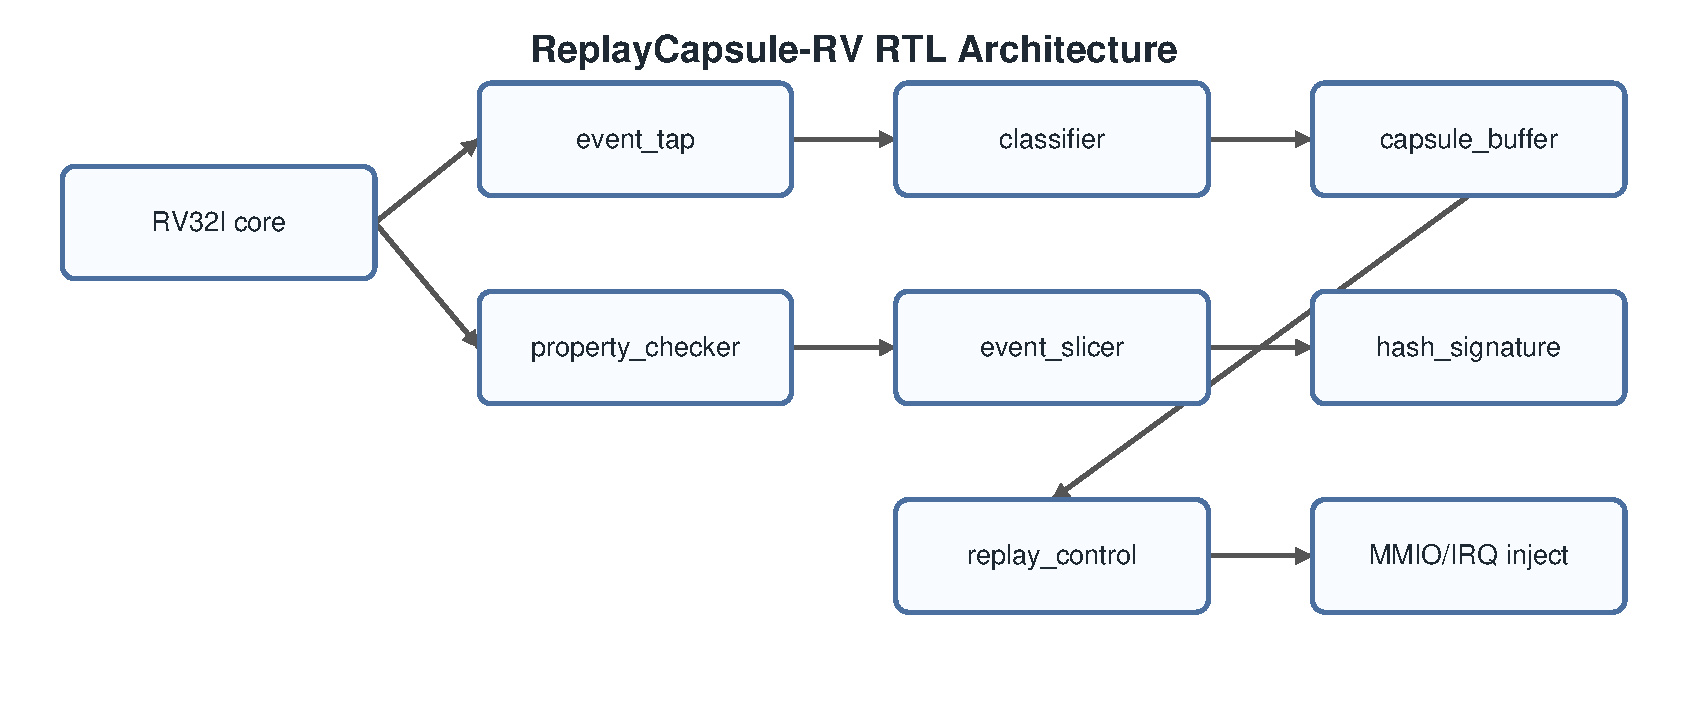
\includegraphics[width=\linewidth]{figures/architecture_overview.pdf}}{\fbox{\parbox{\linewidth}{Generated source: \texttt{paper/figures/architecture\_overview.svg}}}}
\caption{ReplayCapsule hardware architecture. Source generated from \texttt{scripts/make\_figures.py}.}
\label{fig:architecture}
\end{figure}

The board-level mapped wrappers expose only clock, reset, UART, GPIO, status LEDs, and three recorder-status pins. Large debug and internal buses remain inside the FPGA design. The prototype prioritizes replay fidelity and auditability over area minimization; Section~\ref{sec:evaluation} reports the generated same-target ECP5 mapped overhead rather than presenting the recorder as an optimized implementation.
